\let\negmedspace\undefined
\let\negthickspace\undefined
\documentclass[journal]{IEEEtran}
\usepackage[a5paper, margin=10mm, onecolumn]{geometry}
%\usepackage{lmodern} 
\usepackage{tfrupee} 

\setlength{\headheight}{1cm} 
\setlength{\headsep}{0mm}     

\usepackage{gvv-book}
\usepackage{gvv}
\usepackage{cite}
\usepackage{amsmath,amssymb,amsfonts,amsthm}
\usepackage{algorithmic}
\usepackage{graphicx}
\usepackage{textcomp}
\usepackage{xcolor}
\usepackage{txfonts}
\usepackage{listings}
\usepackage{enumitem}
\usepackage{mathtools}
\usepackage{gensymb}
\usepackage{comment}
\usepackage[breaklinks=true]{hyperref}
\usepackage{tkz-euclide} 
\usepackage{listings}                                        
\def\inputGnumericTable{}                                 
\usepackage[latin1]{inputenc}                                
\usepackage{color}                                            
\usepackage{array}                                            
\usepackage{longtable}                                       
\usepackage{calc}                                             
\usepackage{multirow}                                         
\usepackage{hhline}                                           
\usepackage{ifthen}                                           
\usepackage{lscape}

\begin{document}

\bibliographystyle{IEEEtran}
\vspace{3cm}

\title{4.12.8}
\author{AI25BTECH11003 - Bhavesh Gaikwad}
{\let\newpage\relax\maketitle}

\renewcommand{\thefigure}{\theenumi}
\renewcommand{\thetable}{\theenumi}
\setlength{\intextsep}{10pt} 


\numberwithin{equation}{enumi}
\numberwithin{figure}{enumi}
\renewcommand{\thetable}{\theenumi}


\textbf{Question}: Distance of the point $(\alpha, \beta, \gamma)$ from y-axis is\\
a) $\beta$\\
b) $|\beta|$\\
c) $|\beta + \gamma|$\\
d)$\sqrt{\alpha^2 + \gamma^2}$ \\

\textbf{Solution:}\\
Let $\vec{A} = \myvec{\alpha \\ \beta \\ \gamma}$\\ 
Let $\vec{B}$ be an arbitrary point on the y-axis.

\begin{equation}
    \text{Equation of y-axis: } \vec{r} = t\vec{e_2} \, \,
    OR \, \, \vec{r}=t\myvec{0 \\ 1 \\ 0}
\end{equation}

\begin{equation}
\therefore \, \vec{B}=\myvec{0 \\ t \\0}
\end{equation}

\begin{equation}
\text{For minimum distance from y-axis: } \vec{(A-B)} \text{ should be perpendicular to } \vec{e_2}
\end{equation}

\begin{center}
    OR
\end{center}

\begin{equation}
\vec{(A-B)}^T\vec{e_2} =0 \, \Rightarrow \, \myvec{\alpha \\ \beta-t \\ \gamma}^T\myvec{0 \\ 1 \\ 0} = 0     
\end{equation}\\

Therefore, from Equation 0.4,
\begin{equation}
t=\beta
\end{equation}

Therefore the distance between y-axis and $\vec{A}$ is:
\begin{equation}
    \norm{\vec{B-A}}  = \norm{\myvec{\alpha \\ 0 \\ \gamma}} = \sqrt{\alpha^2 + \gamma^2}
\end{equation}

\begin{equation}
\boxed{\text{Therefore, Option D is Correct.}}    
\end{equation}

\begin{figure}[htbp]
    \centering
    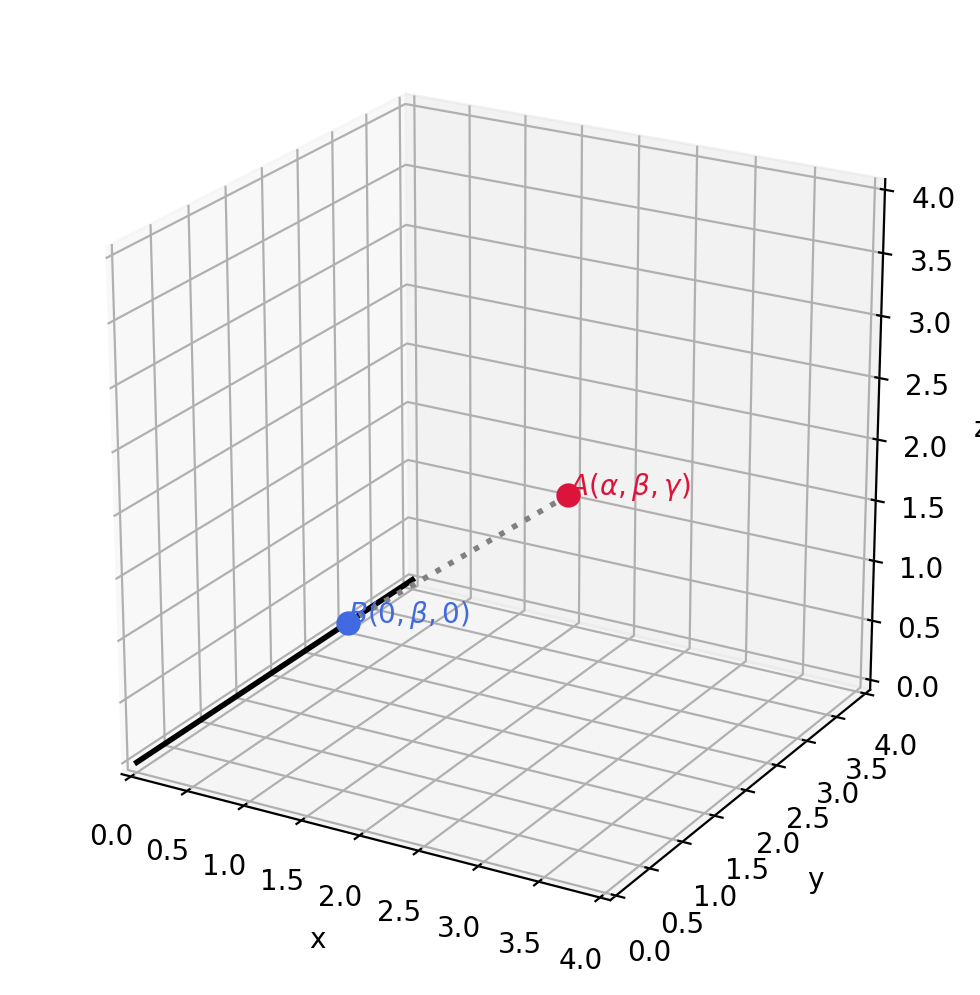
\includegraphics[width=\columnwidth]{figs/fig1.png}
    \caption{Plane}
    \label{fig:fig/fig1.png}
\end{figure}
\end{document}  
